% 9steps
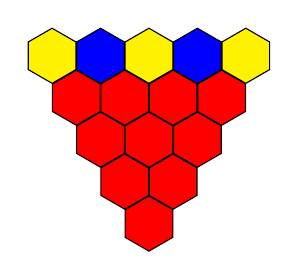
\begin{tikzpicture}[scale=0.35]
  %9段目
  \filldraw[fill=red] (0,0)--++(30:1)--++(90:1)--++(150:1)--++(210:1)--++(270:1)--cycle;
  %8段目
  \filldraw[fill=red,xshift={-25},yshift={25*sqrt(3)}] (0,0)--++(30:1)--++(90:1)--++(150:1)--++(210:1)--++(270:1)--cycle;
  \filldraw[fill=red,xshift={25},yshift={25*sqrt(3)}] (0,0)--++(30:1)--++(90:1)--++(150:1)--++(210:1)--++(270:1)--cycle;
  %7段目
  \filldraw[fill=red,xshift={-25*2},yshift={25*sqrt(3)*2}] (0,0)--++(30:1)--++(90:1)--++(150:1)--++(210:1)--++(270:1)--cycle;
  \filldraw[fill=red,yshift={25*sqrt(3)*2}] (0,0)--++(30:1)--++(90:1)--++(150:1)--++(210:1)--++(270:1)--cycle;
  \filldraw[fill=red,xshift={25*2},yshift={25*sqrt(3)*2}] (0,0)--++(30:1)--++(90:1)--++(150:1)--++(210:1)--++(270:1)--cycle;
  %6段目
  \filldraw[fill=red,xshift={-25*3},yshift={25*sqrt(3)*3}] (0,0)--++(30:1)--++(90:1)--++(150:1)--++(210:1)--++(270:1)--cycle;
  \filldraw[fill=red,xshift={-25},yshift={25*sqrt(3)*3}] (0,0)--++(30:1)--++(90:1)--++(150:1)--++(210:1)--++(270:1)--cycle;
  \filldraw[fill=red,xshift={25},yshift={25*sqrt(3)*3}] (0,0)--++(30:1)--++(90:1)--++(150:1)--++(210:1)--++(270:1)--cycle;
  \filldraw[fill=red,xshift={25*3},yshift={25*sqrt(3)*3}] (0,0)--++(30:1)--++(90:1)--++(150:1)--++(210:1)--++(270:1)--cycle;
  %5段目
  \filldraw[fill=yellow,xshift={-25*4},yshift={25*sqrt(3)*4}] (0,0)--++(30:1)--++(90:1)--++(150:1)--++(210:1)--++(270:1)--cycle;
  \filldraw[fill=blue,xshift={-25*2},yshift={25*sqrt(3)*4}] (0,0)--++(30:1)--++(90:1)--++(150:1)--++(210:1)--++(270:1)--cycle;
  \filldraw[fill=yellow,yshift={25*sqrt(3)*4}] (0,0)--++(30:1)--++(90:1)--++(150:1)--++(210:1)--++(270:1)--cycle;
  \filldraw[fill=blue,xshift={25*2},yshift={25*sqrt(3)*4}] (0,0)--++(30:1)--++(90:1)--++(150:1)--++(210:1)--++(270:1)--cycle;
  \filldraw[fill=yellow,xshift={25*4},yshift={25*sqrt(3)*4}] (0,0)--++(30:1)--++(90:1)--++(150:1)--++(210:1)--++(270:1)--cycle;
\end{tikzpicture}
